\documentclass[border={0.000000bp 0.000000bp 0.000000bp 0.000000bp}, 11pt]{standalone}
\pdfinfoomitdate=1
\pdftrailerid{}
\pdfsuppressptexinfo=1
\pdfinfo{ /Creator () /Producer () }

\usepackage{tikz}
\usepackage{xcolor}
\usetikzlibrary{shapes.misc}
\usetikzlibrary{backgrounds}

\definecolor{dotColorA}{HTML}{000000}
\definecolor{dotColorB}{HTML}{000000}
\definecolor{dotColorC}{HTML}{000000}
\definecolor{dotColorD}{HTML}{000000}
\definecolor{dotColorE}{HTML}{000000}
\definecolor{dotColorF}{HTML}{000000}
\definecolor{dotColorG}{HTML}{000000}
\definecolor{dotColorH}{HTML}{000000}
\definecolor{dotColorI}{HTML}{000000}
\definecolor{dotColorJ}{HTML}{000000}
\definecolor{dotColorK}{HTML}{000000}
\definecolor{dotColorL}{HTML}{000000}
\definecolor{dotColorM}{HTML}{000000}

\definecolor{labelBgColorA}{HTML}{FFFFFF}
\definecolor{labelBgColorB}{HTML}{FFFFFF}
\definecolor{labelBgColorC}{HTML}{FFFFFF}
\definecolor{labelBgColorD}{HTML}{FFFFFF}
\definecolor{labelBgColorE}{HTML}{FFFFFF}
\definecolor{labelBgColorF}{HTML}{FFFFFF}
\definecolor{labelBgColorG}{HTML}{FFFFFF}
\definecolor{labelBgColorH}{HTML}{FFFFFF}
\definecolor{labelBgColorI}{HTML}{FFFFFF}
\definecolor{labelBgColorJ}{HTML}{FFFFFF}
\definecolor{labelBgColorK}{HTML}{FFFFFF}
\definecolor{labelBgColorL}{HTML}{FFFFFF}
\definecolor{labelBgColorM}{HTML}{FFFFFF}

\definecolor{labelTextColorA}{HTML}{000000}
\definecolor{labelTextColorB}{HTML}{000000}
\definecolor{labelTextColorC}{HTML}{000000}
\definecolor{labelTextColorD}{HTML}{000000}
\definecolor{labelTextColorE}{HTML}{000000}
\definecolor{labelTextColorF}{HTML}{000000}
\definecolor{labelTextColorG}{HTML}{000000}
\definecolor{labelTextColorH}{HTML}{000000}
\definecolor{labelTextColorI}{HTML}{000000}
\definecolor{labelTextColorJ}{HTML}{000000}
\definecolor{labelTextColorK}{HTML}{000000}
\definecolor{labelTextColorL}{HTML}{000000}
\definecolor{labelTextColorM}{HTML}{000000}

\definecolor{linkColorA}{HTML}{000000}
\definecolor{linkColorB}{HTML}{000000}
\definecolor{linkColorC}{HTML}{000000}
\definecolor{linkColorD}{HTML}{000000}
\definecolor{linkColorE}{HTML}{000000}
\definecolor{linkColorF}{HTML}{000000}
\definecolor{linkColorG}{HTML}{000000}
\definecolor{linkColorH}{HTML}{000000}
\definecolor{linkColorI}{HTML}{000000}
\definecolor{linkColorJ}{HTML}{000000}
\definecolor{linkColorK}{HTML}{000000}
\definecolor{linkColorL}{HTML}{000000}
\definecolor{linkColorM}{HTML}{000000}

\def\textA{\textsc{amoc}}
\def\textB{\textsc{binseg}}
\def\textC{\textsc{bocpd}}
\def\textD{\textsc{bocpdms}}
\def\textE{\textsc{cpnp}}
\def\textF{\textsc{ecp}}
\def\textG{\textsc{kcpa}}
\def\textH{\textsc{pelt}}
\def\textI{\textsc{prophet}}
\def\textJ{\textsc{rfpop}}
\def\textK{\textsc{segneigh}}
\def\textL{\textsc{wbs}}
\def\textM{\textsc{zero}}

\begin{document}
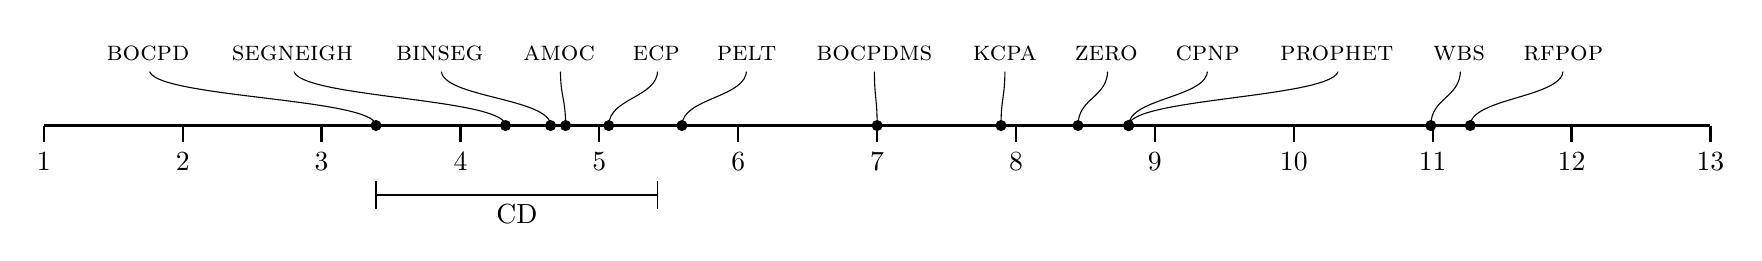
\begin{tikzpicture}[x=1bp,y=-1bp]

% shift for the margin
\begin{scope}[shift={(0, 0)}]
% main layer
\begin{scope}[shift={(0, 75)}]
% axis
\begin{scope}
\draw[very thick] (0, 0) -- (600, 0);
\end{scope}

% axis layer
\begin{scope}
\begin{scope}[shift={(0, 0)}]
\draw[thick] (0, 0) -- (0, -6pt)
node[anchor=north] {1};
\end{scope}
\begin{scope}[shift={(50, 0)}]
\draw[thick] (0, 0) -- (0, -6pt)
node[anchor=north] {2};
\end{scope}
\begin{scope}[shift={(100, 0)}]
\draw[thick] (0, 0) -- (0, -6pt)
node[anchor=north] {3};
\end{scope}
\begin{scope}[shift={(150, 0)}]
\draw[thick] (0, 0) -- (0, -6pt)
node[anchor=north] {4};
\end{scope}
\begin{scope}[shift={(200, 0)}]
\draw[thick] (0, 0) -- (0, -6pt)
node[anchor=north] {5};
\end{scope}
\begin{scope}[shift={(250, 0)}]
\draw[thick] (0, 0) -- (0, -6pt)
node[anchor=north] {6};
\end{scope}
\begin{scope}[shift={(300, 0)}]
\draw[thick] (0, 0) -- (0, -6pt)
node[anchor=north] {7};
\end{scope}
\begin{scope}[shift={(350, 0)}]
\draw[thick] (0, 0) -- (0, -6pt)
node[anchor=north] {8};
\end{scope}
\begin{scope}[shift={(400, 0)}]
\draw[thick] (0, 0) -- (0, -6pt)
node[anchor=north] {9};
\end{scope}
\begin{scope}[shift={(450, 0)}]
\draw[thick] (0, 0) -- (0, -6pt)
node[anchor=north] {10};
\end{scope}
\begin{scope}[shift={(500, 0)}]
\draw[thick] (0, 0) -- (0, -6pt)
node[anchor=north] {11};
\end{scope}
\begin{scope}[shift={(550, 0)}]
\draw[thick] (0, 0) -- (0, -6pt)
node[anchor=north] {12};
\end{scope}
\begin{scope}[shift={(600, 0)}]
\draw[thick] (0, 0) -- (0, -6pt)
node[anchor=north] {13};
\end{scope}
\end{scope}

% link layer
\begin{scope}
\draw[color=linkColorA, thin] (187.83783783783784, 0) .. controls
(187.83783783783784, -10.0) and (186.0, -10.0) .. (186.0, -20.0);
\draw[color=linkColorB, thin] (182.4324324324324, 0) .. controls
(182.4324324324324, -10.0) and (143.0, -10.0) .. (143.0, -20.0);
\draw[color=linkColorC, thin] (119.59459459459461, 0) .. controls
(119.59459459459461, -10.0) and (38.0, -10.0) .. (38.0, -20.0);
\draw[color=linkColorD, thin] (300.0, 0) .. controls
(300.0, -10.0) and (299.0, -10.0) .. (299.0, -20.0);
\draw[color=linkColorE, thin] (390.5405405405406, 0) .. controls
(390.5405405405406, -10.0) and (419.0, -10.0) .. (419.0, -20.0);
\draw[color=linkColorF, thin] (203.37837837837836, 0) .. controls
(203.37837837837836, -10.0) and (221.0, -10.0) .. (221.0, -20.0);
\draw[color=linkColorG, thin] (344.5945945945946, 0) .. controls
(344.5945945945946, -10.0) and (346.0, -10.0) .. (346.0, -20.0);
\draw[color=linkColorH, thin] (229.72972972972974, 0) .. controls
(229.72972972972974, -10.0) and (253.0, -10.0) .. (253.0, -20.0);
\draw[color=linkColorI, thin] (390.5405405405406, 0) .. controls
(390.5405405405406, -10.0) and (466.0, -10.0) .. (466.0, -20.0);
\draw[color=linkColorJ, thin] (513.5135135135135, 0) .. controls
(513.5135135135135, -10.0) and (547.0, -10.0) .. (547.0, -20.0);
\draw[color=linkColorK, thin] (166.21621621621622, 0) .. controls
(166.21621621621622, -10.0) and (90.0, -10.0) .. (90.0, -20.0);
\draw[color=linkColorL, thin] (499.3243243243243, 0) .. controls
(499.3243243243243, -10.0) and (510.0, -10.0) .. (510.0, -20.0);
\draw[color=linkColorM, thin] (372.29729729729723, 0) .. controls
(372.29729729729723, -10.0) and (383.0, -10.0) .. (383.0, -20.0);
\end{scope}

% label layer
\begin{scope}
\begin{scope}[shift={(167, -34)}]
\fill[color=labelBgColorA, rounded corners=2pt]
(0, 0) rectangle (37, 14.62708) node[midway, yshift=-.75bp, anchor=center, text=labelTextColorA] {\strut \textA};
\end{scope}
\begin{scope}[shift={(121, -34)}]
\fill[color=labelBgColorB, rounded corners=2pt]
(0, 0) rectangle (43, 14.62708) node[midway, yshift=-.75bp, anchor=center, text=labelTextColorB] {\strut \textB};
\end{scope}
\begin{scope}[shift={(17, -34)}]
\fill[color=labelBgColorC, rounded corners=2pt]
(0, 0) rectangle (41, 14.62708) node[midway, yshift=-.75bp, anchor=center, text=labelTextColorC] {\strut \textC};
\end{scope}
\begin{scope}[shift={(272, -34)}]
\fill[color=labelBgColorD, rounded corners=2pt]
(0, 0) rectangle (54, 14.62708) node[midway, yshift=-.75bp, anchor=center, text=labelTextColorD] {\strut \textD};
\end{scope}
\begin{scope}[shift={(402, -34)}]
\fill[color=labelBgColorE, rounded corners=2pt]
(0, 0) rectangle (34, 14.62708) node[midway, yshift=-.75bp, anchor=center, text=labelTextColorE] {\strut \textE};
\end{scope}
\begin{scope}[shift={(207, -34)}]
\fill[color=labelBgColorF, rounded corners=2pt]
(0, 0) rectangle (27, 14.62708) node[midway, yshift=-.75bp, anchor=center, text=labelTextColorF] {\strut \textF};
\end{scope}
\begin{scope}[shift={(329, -34)}]
\fill[color=labelBgColorG, rounded corners=2pt]
(0, 0) rectangle (34, 14.62708) node[midway, yshift=-.75bp, anchor=center, text=labelTextColorG] {\strut \textG};
\end{scope}
\begin{scope}[shift={(237, -34)}]
\fill[color=labelBgColorH, rounded corners=2pt]
(0, 0) rectangle (32, 14.62708) node[midway, yshift=-.75bp, anchor=center, text=labelTextColorH] {\strut \textH};
\end{scope}
\begin{scope}[shift={(439, -34)}]
\fill[color=labelBgColorI, rounded corners=2pt]
(0, 0) rectangle (53, 14.62708) node[midway, yshift=-.75bp, anchor=center, text=labelTextColorI] {\strut \textI};
\end{scope}
\begin{scope}[shift={(527, -34)}]
\fill[color=labelBgColorJ, rounded corners=2pt]
(0, 0) rectangle (40, 14.62708) node[midway, yshift=-.75bp, anchor=center, text=labelTextColorJ] {\strut \textJ};
\end{scope}
\begin{scope}[shift={(61, -34)}]
\fill[color=labelBgColorK, rounded corners=2pt]
(0, 0) rectangle (57, 14.62708) node[midway, yshift=-.75bp, anchor=center, text=labelTextColorK] {\strut \textK};
\end{scope}
\begin{scope}[shift={(495, -34)}]
\fill[color=labelBgColorL, rounded corners=2pt]
(0, 0) rectangle (29, 14.62708) node[midway, yshift=-.75bp, anchor=center, text=labelTextColorL] {\strut \textL};
\end{scope}
\begin{scope}[shift={(366, -34)}]
\fill[color=labelBgColorM, rounded corners=2pt]
(0, 0) rectangle (33, 14.62708) node[midway, yshift=-.75bp, anchor=center, text=labelTextColorM] {\strut \textM};
\end{scope}
\end{scope}

% dots
\begin{scope}
\draw node [circle, inner sep=0pt, minimum size=4bp, 
fill=dotColorA] at (187.837838, 0) {};
\draw node [circle, inner sep=0pt, minimum size=4bp, 
fill=dotColorB] at (182.432432, 0) {};
\draw node [circle, inner sep=0pt, minimum size=4bp, 
fill=dotColorC] at (119.594595, 0) {};
\draw node [circle, inner sep=0pt, minimum size=4bp, 
fill=dotColorD] at (300.000000, 0) {};
\draw node [circle, inner sep=0pt, minimum size=4bp, 
fill=dotColorE] at (390.540541, 0) {};
\draw node [circle, inner sep=0pt, minimum size=4bp, 
fill=dotColorF] at (203.378378, 0) {};
\draw node [circle, inner sep=0pt, minimum size=4bp, 
fill=dotColorG] at (344.594595, 0) {};
\draw node [circle, inner sep=0pt, minimum size=4bp, 
fill=dotColorH] at (229.729730, 0) {};
\draw node [circle, inner sep=0pt, minimum size=4bp, 
fill=dotColorI] at (390.540541, 0) {};
\draw node [circle, inner sep=0pt, minimum size=4bp, 
fill=dotColorJ] at (513.513514, 0) {};
\draw node [circle, inner sep=0pt, minimum size=4bp, 
fill=dotColorK] at (166.216216, 0) {};
\draw node [circle, inner sep=0pt, minimum size=4bp, 
fill=dotColorL] at (499.324324, 0) {};
\draw node [circle, inner sep=0pt, minimum size=4bp, 
fill=dotColorM] at (372.297297, 0) {};
\end{scope}

% Critical difference
\def\posBest{119.5945945945946107}
\def\posCD{221.0672691045307090}
\begin{scope}
\draw (\posBest, 30) -- (\posBest, 20);
\draw (\posBest, 25) --node[below] {CD} (\posCD, 25);
\draw (\posCD, 30) -- (\posCD, 20);
\end{scope}

\end{scope}
\end{scope}
\end{tikzpicture}
\end{document}